\documentclass[11pt,a4paper]{article}

\usepackage[margin=2.5cm]{geometry}
\usepackage{amsmath,amssymb}
\usepackage{booktabs}
\usepackage{array}
\usepackage{tikz}
\usetikzlibrary{arrows.meta,positioning,calc}
\usepackage[colorlinks=true,linkcolor=blue!50!black,urlcolor=blue!50!black]{hyperref}

\setlength{\emergencystretch}{3em}
\newcommand{\ts}{\mathrm{s}}
\newcommand{\rads}{\,\mathrm{rad/s}}
\newcommand{\radss}{\,\mathrm{rad/s^2}}

\title{Design of a Balancing Controller for a Wheeled Biped Robot\\
\large ROS\,2 / Gazebo Simulation with Velocity-Commanded Wheels}
\author{ROS2-Bipedbot project}
\date{\today}

\begin{document}
\maketitle

\begin{abstract}
This report documents how the balancing controller of the bipedbot was
designed and why it has its present structure. The robot is a wheeled
inverted pendulum whose wheels accept a \emph{velocity} command. A direct PD
law from tilt angle to wheel velocity cannot stabilise such a plant at any
gain; the controller therefore treats the PID output as wheel
\emph{acceleration} (integrated into the speed command), and adds a slow
outer loop on wheel speed that finds the true balance angle and prevents
speed run-away. Each stage is derived with a simplified model, compared with
the observed simulation behaviour, and tied to a commit in the repository.
\end{abstract}

\tableofcontents
\newpage

%--------------------------------------------------------------------
\section{System description}
%--------------------------------------------------------------------
The robot balances on two wheels. The relevant interfaces are:

\begin{itemize}
  \item \textbf{Sensor:} a Gazebo IMU at $100\,\mathrm{Hz}$, bridged to ROS\,2 as
        \texttt{/imu/out} (\texttt{sensor\_msgs/Imu}) with orientation,
        angular velocity and linear acceleration.
  \item \textbf{Actuation:} a \texttt{JointGroup\allowbreak Velocity\allowbreak Controller}
        (\texttt{simple\_\allowbreak velocity\_\allowbreak controller}) that takes
        $[\omega_L,\ \omega_R]$ wheel velocity commands, limited to
        $\pm 20\rads$.
  \item \textbf{Geometry:} the wheel axle lies along the body $x$-axis, so the
        wheels can only correct tilt about $x$ (the IMU \emph{roll}). The two
        wheel joints have \emph{mirrored} axes (left $-x$, right $+x$), so
        identical commands spin the wheels in opposite physical directions.
\end{itemize}

The mirrored axes are handled by a sign vector in the command,
\begin{equation}
  \begin{bmatrix}\omega_L\\ \omega_R\end{bmatrix}
  = \begin{bmatrix}-1\\ +1\end{bmatrix}\omega ,
  \label{eq:wheelmap}
\end{equation}
where $\omega$ is the common wheel speed in the ``balancing'' direction.

%--------------------------------------------------------------------
\section{Sensing}
%--------------------------------------------------------------------
The tilt angle $\theta$ is the roll of the IMU orientation quaternion
$(q_x,q_y,q_z,q_w)$:
\begin{equation}
  \theta = \operatorname{atan2}\!\bigl(2(q_w q_x + q_y q_z),\; 1 - 2(q_x^2+q_y^2)\bigr).
  \label{eq:roll}
\end{equation}
The tilt rate $\dot\theta$ is taken directly from the gyroscope
(angular velocity about $x$) rather than by differentiating $\theta$. The gyro
noise is small (simulated $\sigma = 2\times10^{-4}\rads$), whereas a numerical
derivative of the angle amplifies noise at $100\,\mathrm{Hz}$.

%--------------------------------------------------------------------
\section{Plant model}
%--------------------------------------------------------------------
For small tilts, the robot is modelled as a point-mass inverted pendulum of
effective length $l$ on a base (the axle) that accelerates horizontally with
$a$. Let $\theta_0$ be the angle at which the centre of mass lies exactly above
the axle (the \emph{balance angle}). Then
\begin{equation}
  l\,\ddot\theta = g\,(\theta-\theta_0) - a ,
  \label{eq:pendulum}
\end{equation}
and, with no wheel slip and wheel radius $r$,
\begin{equation}
  a = r\,\dot\omega .
  \label{eq:accel}
\end{equation}

Equation~\eqref{eq:pendulum} shows the two key properties of the plant:
\begin{enumerate}
  \item It is \textbf{unstable}: the $g(\theta-\theta_0)/l$ term pushes the tilt
        away from $\theta_0$ (open-loop pole at $+\sqrt{g/l}$).
  \item The only input is the \textbf{wheel acceleration} $\dot\omega$. Gravity can
        only be countered by accelerating the wheels in the direction of the lean.
\end{enumerate}

\paragraph{Assumptions.} Wheel and body inertia, tyre compliance, and
actuator dynamics are neglected, and the wheels are assumed to follow velocity
commands almost ideally. The effective length $l$, the wheel radius $r$ and
the balance angle $\theta_0$ were \emph{not} measured; the design below is
therefore tuned experimentally and the model is used to explain structure, not
to compute final gains.

%--------------------------------------------------------------------
\section{Controller design}
%--------------------------------------------------------------------
Throughout, $e = \theta - \theta_\mathrm{ref}$ and $u$ is the PID output.

\subsection{Stage 1: PD output used as wheel velocity (cannot work)}
\label{sec:stage1}
The first design set the wheel velocity directly:
\begin{equation}
  \omega = u = k_p\,e + k_d\,\dot\theta .
  \label{eq:stage1}
\end{equation}
Then $\dot\omega = k_p\dot\theta + k_d\ddot\theta$, and
\eqref{eq:pendulum}--\eqref{eq:accel} give
\begin{equation}
  (l + r k_d)\,\ddot\theta + r k_p\,\dot\theta - g\,(\theta-\theta_0) = 0 .
\end{equation}
The characteristic polynomial is
\begin{equation}
  (l + r k_d)\,s^2 + r k_p\,s - g = 0 .
\end{equation}
Its constant term is negative while the leading coefficient is positive, so the
product of the roots is negative: there is always one root in the right
half-plane, \textbf{for any gains}. A velocity command is the integral of
wheel acceleration, so a PD law on angle yields an acceleration proportional
to $\dot\theta$ and $\ddot\theta$, but never to $\theta$ itself, and the
$\theta$ term is exactly what must overcome gravity.

\emph{Observed:} the robot fell in about $0.7\,\mathrm{s}$ regardless of the
gains tried.

\subsection{Stage 2: PID output as wheel acceleration}
\label{sec:stage2}
The fix is to interpret $u$ as wheel \emph{acceleration} and integrate it into
the speed command:
\begin{equation}
  u = k_p\,e + k_i\!\int e\,dt + k_d\,\dot\theta, \qquad
  \dot\omega = u .
  \label{eq:stage2}
\end{equation}
With $k_i = 0$ the closed loop is
\begin{equation}
  l\,\ddot\theta + r k_d\,\dot\theta + (r k_p - g)\,\theta
  = r k_p\,\theta_\mathrm{ref} - g\,\theta_0 ,
\end{equation}
which is a damped second-order system. It is stable if and only if
\begin{equation}
  k_p > \frac{g}{r}, \qquad k_d > 0 ,
  \label{eq:stability}
\end{equation}
with natural frequency and damping ratio
\begin{equation}
  \omega_n = \sqrt{\frac{r k_p - g}{l}}, \qquad
  \zeta = \frac{r k_d}{2\sqrt{l\,(r k_p - g)}} .
\end{equation}
The $k_p$ bound has the practical meaning that the wheels must accelerate
faster than gravity can make the base ``fall away''. For an
\emph{assumed} wheel radius of $r = 0.05\,\mathrm{m}$ (not measured),
$g/r \approx 196\,\mathrm{s^{-2}}$, which is why gains of order $60$ failed
and $k_p = 400$ worked.

\emph{Observed:} with $k_p = 400$, $k_d = 20$ and $\theta_\mathrm{ref}=-0.03$
the robot held its angle for about three seconds.

\subsection{Why Stage 2 still fails: the setpoint offset}
\label{sec:offset}
If $\theta_\mathrm{ref} \neq \theta_0$, the loop settles to a state with
constant wheel acceleration. Setting $\ddot\theta=\dot\theta=0$ in
\eqref{eq:pendulum} with $a = r k_p(\theta-\theta_\mathrm{ref})$ gives
\begin{equation}
  e^{*} = \frac{g\,(\theta_\mathrm{ref}-\theta_0)}{r k_p - g},
  \qquad
  \dot\omega^{*} = k_p\,e^{*} = K\,(\theta_\mathrm{ref}-\theta_0),
  \qquad
  K = \frac{g\,k_p}{r k_p - g} > 0 .
  \label{eq:steady}
\end{equation}
A tiny setpoint error therefore produces a constant wheel acceleration, and the
wheel speed ramps linearly, $\omega(t)=\dot\omega^{*}t$, until it hits the
actuator limit. The error is small ($\approx 0.03$--$0.05\,\mathrm{rad}$ in the
experiments, invisible on a plot scaled to $\pm20$), but it is
unobservable only until the speed saturates and the wheels lose authority.

Equation~\eqref{eq:steady} also shows a non-intuitive sign: a setpoint
\emph{below} the balance angle ($\theta_\mathrm{ref} < \theta_0$) drives the
speed \emph{negative}, so the correction must raise the setpoint.

\emph{Observed:} the speed ramped to the $-20\rads$ clamp at roughly
$-20\radss$ and the robot then fell.

\subsection{Stage 3: outer speed loop}
\label{sec:stage3}
A second, slower loop adds a lean offset $\delta$ to the reference, driven by
the wheel speed:
\begin{equation}
  \delta = -k_{v,p}\,\omega + \tau, \qquad \dot\tau = -k_{v,i}\,\omega,
  \qquad
  \theta_\mathrm{ref,eff} = \theta_\mathrm{ref} + \delta .
  \label{eq:outer}
\end{equation}
Negative speed raises the target lean, so the robot accelerates back toward
zero speed. If the inner loop is fast compared with the outer loop, it can be
replaced by its steady-state map \eqref{eq:steady}:
\begin{equation}
  \dot\omega = K\,(\theta_\mathrm{ref} - \theta_0 + \delta).
\end{equation}
Differentiating and substituting \eqref{eq:outer},
\begin{equation}
  \ddot\omega + K k_{v,p}\,\dot\omega + K k_{v,i}\,\omega = 0 ,
  \label{eq:outerdyn}
\end{equation}
which is stable for $k_{v,p},k_{v,i}>0$, with
\begin{equation}
  \omega_o = \sqrt{K k_{v,i}}, \qquad
  \zeta_o = \frac{K k_{v,p}}{2\sqrt{K k_{v,i}}} .
\end{equation}
In steady state $\omega \to 0$, $\dot\omega=0$, hence
\begin{equation}
  \tau_\infty = \theta_0 - \theta_\mathrm{ref} .
  \label{eq:trim}
\end{equation}
The integral term therefore \emph{identifies the balance angle}:
$\theta_0 = \theta_\mathrm{ref} + \tau_\infty$.

\paragraph{Numerical illustration.} For the same assumed $r = 0.05\,\mathrm{m}$
and $k_p = 400\,\mathrm{s^{-2}}$, $K \approx 385\,\mathrm{s^{-2}}$. With
$k_{v,p}=0.003\,\mathrm{s}$, $k_{v,i}=5\times10^{-4}$ one gets
$\omega_o \approx 0.44\rads$ and $\zeta_o \approx 1.3$, a slow, well-damped
outer loop. With $k_{v,p}=0.01$, $k_{v,i}=0.005$, $\omega_o \approx 1.4\rads$:
the outer loop moves close to the inner-loop bandwidth, the time-scale
separation behind \eqref{eq:outerdyn} weakens, and combined with speed
saturation this is consistent with the limit cycle seen in simulation
(Section~\ref{sec:results}). The model does not predict that limit cycle
quantitatively; it only indicates why the outer loop must be kept slow.

\begin{figure}[ht]
\centering
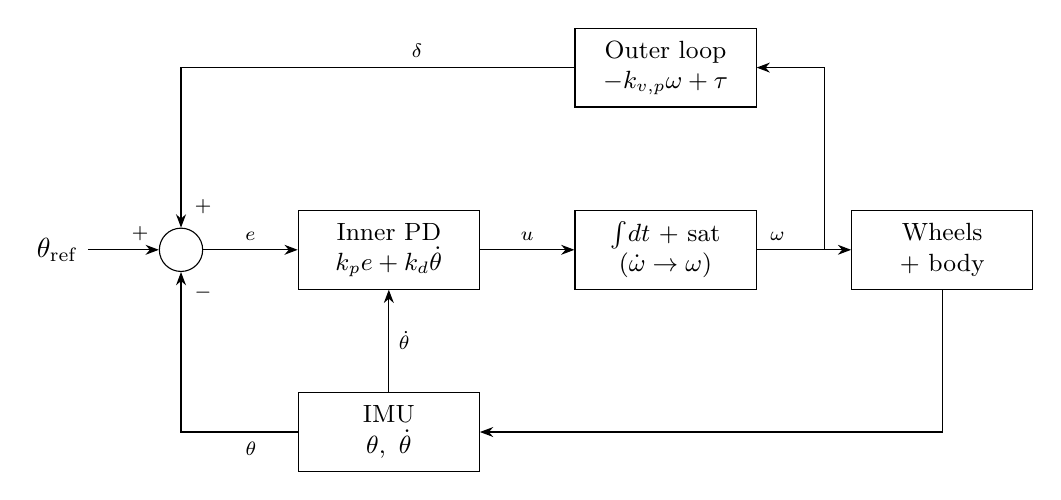
\begin{tikzpicture}[
  node distance=1.5cm and 1.2cm,
  block/.style={draw, rectangle, minimum height=1.0cm, minimum width=2.3cm,
                align=center, font=\small},
  sum/.style={draw, circle, minimum size=0.55cm, inner sep=0pt, font=\small},
  >=Stealth]
  \node (ref) {$\theta_\mathrm{ref}$};
  \node[sum, right=0.9cm of ref] (s1) {};
  \node[block, right=of s1] (pd) {Inner PD\\ $k_p e + k_d\dot\theta$};
  \node[block, right=of pd] (int) {$\int\!dt$ + sat\\ ($\dot\omega\to\omega$)};
  \node[block, right=of int] (pl) {Wheels\\ + body};
  \node[block, above=1.3cm of int] (outer) {Outer loop\\ $-k_{v,p}\omega+\tau$};
  \node[block, below=1.3cm of pd] (imu) {IMU\\ $\theta,\ \dot\theta$};

  \draw[->] (ref) -- (s1);
  \draw[->] (s1) -- node[above, font=\scriptsize]{$e$} (pd);
  \draw[->] (pd) -- node[above, font=\scriptsize]{$u$} (int);
  \draw[->] (int) -- node[above, pos=0.22, font=\scriptsize]{$\omega$} (pl);
  \draw[->] ($(int.east)!0.72!(pl.west)$) |- (outer);
  \draw[->] (outer) -| node[above, pos=0.2, font=\scriptsize]{$\delta$} (s1);
  \draw[->] (pl.south) |- (imu.east);
  \draw[->] (imu.north) -- node[right, font=\scriptsize]{$\dot\theta$} (pd.south);
  \draw[->] (imu.west) -| node[below, pos=0.2, font=\scriptsize]{$\theta$} (s1.south);
  \node[font=\scriptsize] at ($(s1)+(-0.52,0.2)$) {$+$};
  \node[font=\scriptsize] at ($(s1)+(0.28,0.55)$) {$+$};
  \node[font=\scriptsize] at ($(s1)+(0.28,-0.55)$) {$-$};
\end{tikzpicture}
\caption{Cascaded structure. The inner loop produces wheel acceleration from
tilt; the outer loop adjusts the lean target from wheel speed.}
\label{fig:block}
\end{figure}

\subsection{Discrete implementation}
The node runs at the IMU rate ($\approx100\,\mathrm{Hz}$) with $\Delta t_k$ taken
from the message timestamps (samples with $\Delta t\le0$ or $\Delta t>0.1\,\mathrm{s}$ are
skipped). Per cycle:
\begin{align}
  e_k &= \theta_k - \bigl(\theta_\mathrm{ref} + \delta_k\bigr), \\
  u_k &= k_p e_k + k_i I_k + k_d \dot\theta_k, \\
  \omega_{k+1} &= \operatorname{sat}_{\pm\omega_\mathrm{max}}\!\bigl(\omega_k + u_k\,\Delta t_k\bigr), \\
  \tau_{k+1} &= \operatorname{sat}_{\pm\delta_\mathrm{max}}\!\bigl(\tau_k - k_{v,i}\,\omega_k\,\Delta t_k\bigr), \\
  \delta_{k+1} &= \operatorname{sat}_{\pm\delta_\mathrm{max}}\!\bigl(\tau_{k+1} - k_{v,p}\,\omega_{k+1}\bigr).
\end{align}
Clamping the integrators gives anti-windup. A safety cutoff zeroes the command
and resets all states when $|\theta-\theta_\mathrm{ref}| > 0.7\,\mathrm{rad}$,
so the wheels do not thrash a fallen robot. All gains are ROS parameters read
every cycle for live tuning.

\begin{table}[ht]
\centering
\caption{Final parameters (defaults in \texttt{balance\_pid.py}).}
\begin{tabular}{@{}llll@{}}
\toprule
Parameter & Symbol & Value & Unit \\
\midrule
\texttt{setpoint}     & $\theta_\mathrm{ref}$ & $-0.005$ & rad \\
\texttt{kp}           & $k_p$ & $400$ & $\mathrm{s^{-2}}$ \\
\texttt{kd}           & $k_d$ & $20$ & $\mathrm{s^{-1}}$ \\
\texttt{ki}           & $k_i$ & $0$ & -- \\
\texttt{speed\_kp}    & $k_{v,p}$ & $0.003$ & s \\
\texttt{speed\_ki}    & $k_{v,i}$ & $5\times10^{-4}$ & -- \\
\texttt{output\_limit}& $\omega_\mathrm{max}$ & $20$ & rad/s \\
\texttt{lean\_limit}  & $\delta_\mathrm{max}$ & $0.2$ & rad \\
\texttt{fall\_angle}  & -- & $0.7$ & rad \\
\texttt{left\_sign}, \texttt{right\_sign} & -- & $-1,\ +1$ & -- \\
\bottomrule
\end{tabular}
\end{table}

%--------------------------------------------------------------------
\section{Experimental results}
\label{sec:results}
%--------------------------------------------------------------------
All runs are in Gazebo with the robot spawned upright. Values are read from
PlotJuggler plots of \texttt{/balance/debug} and are therefore approximate.

\begin{table}[ht]
\centering
\caption{Controller stages and observed behaviour.}
\small
\begin{tabular}{@{}p{1.6cm}p{4.3cm}p{7.3cm}@{}}
\toprule
Stage & Setting & Observation \\
\midrule
1 & PD $\to$ velocity, $k_p{=}60$, $k_d{=}3$ &
  Error grew monotonically from $\approx0.04$ to $0.7\,\mathrm{rad}$ in about
  $0.7\,\mathrm{s}$; command saturated; robot fell. \\
2 & Integrated, $k_p{=}400$, $k_d{=}20$, $\theta_\mathrm{ref}{=}-0.03$ &
  Angle held for about $3\,\mathrm{s}$; wheel speed ramped to the
  $-20\rads$ clamp at roughly $-20\radss$; robot then fell. \\
3a & + outer loop, $k_{v,p}{=}0.01$, $k_{v,i}{=}0.005$ &
  Wheel speed alternated between the $\pm20\rads$ clamps (limit cycle,
  period $\approx1.3\,\mathrm{s}$); error swung by several tenths of a
  radian; robot fell or was near falling. \\
3b & + outer loop, $k_{v,p}{=}0.003$, $k_{v,i}{=}5{\times}10^{-4}$ &
  Stable. Lean offset converged to $\tau_\infty\approx+0.026\,\mathrm{rad}$,
  giving $\theta_0 \approx -0.03+0.026 = -0.004\,\mathrm{rad}$
  via \eqref{eq:trim}. Wheel speed $\approx 0.002\rads$ at rest over the
  observation interval. After a disturbance the speed rang at about
  $1\,\mathrm{Hz}$ with roughly $28\%$ amplitude loss per cycle. \\
\bottomrule
\end{tabular}
\end{table}

The identified balance angle $\theta_0\approx-0.004\,\mathrm{rad}$ is
repeatable across runs ($\tau_\infty = 0.025$--$0.026$), and the final
default $\theta_\mathrm{ref}=-0.005$ is chosen to match it so that the outer
loop starts nearly trimmed. The experimental observations agree
qualitatively with the model: no stabilisation at any gain for Stage~1,
a constant-acceleration run-away for a mis-set reference in Stage~2, and
convergence of $\tau$ to $\theta_0-\theta_\mathrm{ref}$ in Stage~3.

%--------------------------------------------------------------------
\section{Integration problems and fixes}
%--------------------------------------------------------------------
Several failures during development were infrastructure issues rather than
control issues, and masked the control behaviour until fixed.

\begin{table}[ht]
\centering
\caption{Symptoms, causes and fixes.}
\small
\begin{tabular}{@{}p{4.1cm}p{5.2cm}p{4.2cm}@{}}
\toprule
Symptom & Cause & Fix \\
\midrule
\texttt{ros2 topic echo /imu} empty; data on \texttt{/imu/out} &
  Bridge remaps \texttt{/imu} to \texttt{/imu/out} & Use \texttt{/imu/out} \\
Robot fell as if the node were off &
  Commands published to a topic with no subscriber (wrong controller name) &
  Publish to \texttt{/simple\_\allowbreak velocity\_\allowbreak controller/\allowbreak commands} \\
No controllers loaded after a world reset &
  Resetting Gazebo (Ctrl+R) drops the controllers; one-shot spawners do not
  reload them & Restart the simulation instead of resetting \\
Robot turned in place on equal commands &
  Mirrored wheel joint axes in the URDF & $\omega_L=-\omega$, $\omega_R=+\omega$ \\
Fell with any gains, either sign &
  Velocity-command PD has no restoring term (Section~\ref{sec:stage1}) &
  Integrate the PID output (Section~\ref{sec:stage2}) \\
Ran to $\pm20\rads$ after $\approx3\,\mathrm{s}$ &
  Setpoint offset (Section~\ref{sec:offset}) & Outer speed loop \\
Limit cycle after raising $k_d$ &
  The run omitted the outer-gain flags, so the aggressive defaults applied &
  Safe outer gains made the defaults \\
\bottomrule
\end{tabular}
\end{table}

%--------------------------------------------------------------------
\section{Limitations and future work}
%--------------------------------------------------------------------
\begin{itemize}
  \item The plant model is simplified, and $r$, $l$ and the inertias were not
        identified. The stability bound \eqref{eq:stability} and the outer-loop
        numbers are illustrations under an assumed radius, not verified
        predictions.
  \item Gains were tuned by experiment. A state-space design such as LQR
        on the full cart--pendulum model, using identified parameters, would
        give a principled alternative to the cascaded PID.
  \item The controller regulates tilt and wheel speed only. Position and
        heading are uncontrolled, so the robot can drift and yaw freely.
  \item Planned extensions: a \texttt{cmd\_vel} interface (forward speed through
        the lean offset, yaw through a differential wheel term), and starting
        the node from the simulation launch file.
\end{itemize}

%--------------------------------------------------------------------
\appendix
\section{Mapping to repository commits}
%--------------------------------------------------------------------
\begin{table}[ht]
\centering
\caption{Development stages and commits.}
\small
\begin{tabular}{@{}lp{9.6cm}@{}}
\toprule
Commit & Content \\
\midrule
\texttt{0400c38} & Simulation interface: ros2\_control wheels, IMU sensor, ROS bridge \\
\texttt{3a1b956} & \texttt{bipedbot\_controller} package with wheel velocity controller \\
\texttt{c84072c} & Stage 1: PD on tilt commanding wheel velocity \\
\texttt{9febfe9} & Stage 2: PID output as wheel acceleration, integrated to speed \\
\texttt{b07beed} & Stage 3: wheel-speed outer loop and tuned defaults \\
\bottomrule
\end{tabular}
\end{table}

\section{Tuning guide}
\begin{enumerate}
  \item Verify the wheel signs: equal commands should drive the robot straight
        (opposite physical wheel directions are corrected by
        \eqref{eq:wheelmap}).
  \item Raise $k_p$ until the robot holds a lean; it must exceed $g/r$.
  \item Add $k_d$ until post-disturbance ringing decays; reduce it if the
        command buzzes at high frequency.
  \item Enable the outer loop with small gains. If the speed still runs away
        monotonically, the outer-loop sign is wrong; if it swings between the
        limits, the outer gains are too high.
  \item Read $\tau_\infty$ from \texttt{/balance/debug} and fold it into
        \texttt{setpoint}.
\end{enumerate}

\end{document}
